%!TEX root = ../MAsterthesis.tex
\chapter{Tracking in real space}
The previous sections provided information on the structure of the human hand and how to represent it in the digital space. To apply the algorithms presented in Section \ref{kinematics} to our digital hand model, we need input data from our real world representative.\\The methods for gaining positional data can be roughly categorized into two major groups, glove based methods and vision based methods. Glove based methods have already been in developement since the 1980's \cite{Bolt.1980} and have since then resulted in several solution attempts. Sturman and Zeltzer gave a survey on the exsisting tracking mehtods in their paper \cite{Sturman.1994b}. \\They distinguish between two areas of tracking, first the  3D positional tracking of the hand (and also other bodyparts) without regard to the hands shape and secondly the tracking of the hand shape with glove technologies.\\These tracking technologies presented are still applied today in modern tracking solutions \cite{Welch.2002}. They account for solutions based in optical tracking based on marker detection, magnetic detection via measurements of an artificial megnetic field\cite{Raab.1979} and accoustic measurements via triangulaton of ultrasonic pings.

\subsubsection{Optical tracking}

The components for an optical tracking systems are several cameras for object detection and some kind of tracking characteristic of the object to be tracked. These characteristics can be either artificially applied ones like active flashing infrared LED on key tracking positions of the body or infrared reflective markers.\\ A series of cameras positioned around the tracking subject will then track these markers inside their visual fields. The second method uses a single camera to capture the silhouette image of the subject, which is analyzed to determine positions of the various parts of the body and user gestures.
\\The image data is supplied to special software which correlates the marker positions in the multiple viewpoints and uses the different lens perspectives to calculate a 3D coordinate for each marker. These image interpretation and correlation tasks require computationally costly operations. The marker tracking is also prone to errors through variation in lighting of the scene, material reflection properties and also marker occlusion as the trackers are moved. Also most of the systems rely on several tracking cameras for a complete coverage of the tracking space. This leads to a higher system complexity in terms of setup and calibration.
\begin{figure}[H]
\label{optic reflector tracking}
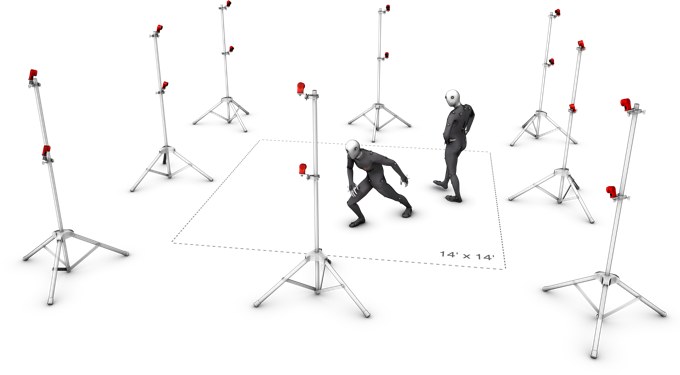
\includegraphics[scale=0.6]{images/flex13MocapVolume.png} 
\caption{Example for an optical tracking system with passive infrared reflector markers \cite{optitrack.2017}}
\end{figure}
\subsubsection{Magnetic tracking}
The usage of a magnetic field for position tracking is a relatively uncomlicated technique. The earth already provides us with a magnetic field to orient on. Simular to the optical trackers, magnet field sensors can be placed at key tracking positions. These sensors measure field strength in 3 orthogonally orented axes to produce a 3D vector of the unit’s orientation with respect to the excitation. As the earths magnetic field prone to changes based on geographical location, data corrections have to be applied to the measurements.\\Another solution is to generate an local magnetic field via a multicoil source unit. The source unit coils are energized in sequence and the corresponding magnetic field vector is measured in the sensor unit. With three such excitations, you can estimate the position and orientation of the sensor unit with respect to the source unit.\\the downside of this technology is that ferromagnetic and conductive material in the surrounding environement will have an effect on the generated magnetic field. These distortion effects will form small unwanted secondary source units through the induction of small Foucault currents by the main sources magnetic field.
Magnetic fields have the property of having an inverse cubic falloff  as a function of distance from the source, which limits the rango of operation for the system.
Position resolution in the radial direction from source to sensor depends on the gradient of the magnetic field strength, and thus the positional jitter grows as the fourth power of the separation distance.\\
In comparison to other tracking technologies, the magnetic field tracking solution has the conveniece of not suffering from line of sight problems from tracker occlusion. The magnetic fields are capable of passing through the human body. Also the sensor size for measuring magnetic fields is rather small, giving the trackers a small volume. Furthermore, only one source unit is needed for the tracking of multiple sensor units.
\subsubsection{Accoustic tracking}
The principles of accoustic tracking are very simular to those of the optic tracking technologies. Instead of using lightwaves, the systems utilize acoustic pulses of ultrasonic wavelenghts to time the time of flight between emitter and sensor for range measurement. To get a good measuring result from the systems, the used accoustic transducerst have to be as omnidirectional as possible,so that the signal can be detected no matter how the emitter is positioned or oriented in the tracking volume. For the speakers to acchieve a wide beam width, their size has to be small.\\ To be able to build the microphones into the tracker, they can only have active surfaces a few millimeters in diameter. This leads to a reduction in range as the efficiency of accoustic transducers is proportial to the active surface area. Also accoustic systems can have problems with ambient noises occluding the signal. This becomes even mor critical when using such a system outdoors.\\Soundwaves travel at a much slower speed than lightwaves which brings benefits and downsides with it. Soundwaves can be reflected from objects, producing so echos which arrive at the recieving sensor at a later point in time. Here the slower speed can be beneficial as we can await the first sound occurence to arrive at the sensor and filter out all later reflections from the data. The reflections of the previous pluse also have to be subsided before a new measurement can be made, lowering the uodate rates of the system. The air the soundwaves travel through is also a limiting factor as humidity, airpressure and air currents can influence the travelling soundwaves.In comparison to the optical systems, the accoustic systems are not as prone to occlusion errors since soundwaves have a better ability to bend around obstacles  than lightwaves.
\\Most of these downside can be adressed with a combination of these systems with another form of tracking like in \cite{Foxlin.1998}.







